\documentclass[12pt]{article}
\usepackage{setspace}
\usepackage{mathtools}
\usepackage{nicefrac}
\usepackage{fullpage}
\usepackage{times}
\usepackage{mathptmx}
\usepackage{amsmath}
\usepackage{graphicx}
\usepackage{pdfpages}
\usepackage{natbib}
\usepackage{listings}
\usepackage{float}
\usepackage{wrapfig}
\usepackage{booktabs}
\usepackage{lscape}
\usepackage{hyperref}
\usepackage{geometry}
\usepackage{longtable}
\usepackage{pdflscape}
\usepackage[affil-it]{authblk}
\usepackage{todonotes}
%\usepackage[latin1]{inputenc}
\usepackage{tikz}
\usetikzlibrary{shapes,arrows,positioning}
\usepackage{amsmath}
\usetikzlibrary{arrows}
\usepackage{caption, subcaption}
\usepackage{subfiles}
%setup hyperlinks color
\usepackage{color}
\definecolor{PSU}{RGB}{0,0,153}
\hypersetup{
	colorlinks=true,       % false: boxed links; true: colored links
	linkcolor=black,          % color of internal links (change box color with linkbordercolor)
	citecolor=PSU,        % color of links to bibliography
	filecolor=PSU,      % color of file links
	urlcolor=PSU           % color of external links
}


\title{Measuring Judicial Independence in the American States: A Latent Variable Approach}

\author{\href{mailto:Jeremy.Johnson@psu.edu}{Jeremy R.\ Johnson}\thanks{All data and code required for replication is available on GitHub at: \url{https://github.com/jrjohnson0821/stateslatentreplication}}}
\affil{Pennsylvania State University}
\date{\today}

\begin{document}
\maketitle
\thispagestyle{empty}
	
\begin{abstract}
Judicial independence and judicial accountability are commonly understood to exist in tension with one another. Many scholars and professionals, among them the American Bar Association, believe that the judiciary should be entirely independent from any outside influence, be it electoral, executive, or legislative. A contrary view is that judges have become too independent, and need to be “reigned in” by those who can affect control over them, primarily through judicial elections. The core of this disagreement lies with differing understandings of what constitutes “independence” and “accountability.” Absent clear conceptualization and measurement of these concepts, much of the normative debate over judicial independence reduces to disagreement over terms. Despite its manifest importance, there is not currently a comprehensive measure of \textit{de jure} judicial independence in American or comparative politics. I develop and use a latent-variable model to score states' \textit{de jure} judicial independence. This measure will be useful in future studies of judicial independence which focus on \textit{de facto} judicial independence.
\end{abstract}
	
	
\pagebreak\doublespacing
\setcounter{page}{1}

\section*{Introduction}\label{Intro}
% A Paragraph
For more than two centuries, judicial institutions have played a key role in the operation of democratic systems of government.  An independent court ``counteracts the logic of `winner-takes-all' where whoever wins the election wins everything. Thanks to the mechanism of constitutional adjudication, the electoral victory is not an `all or nothing' game'' \citep[1685]{Ferejohn2003}. Normatively, courts provide a secondary outlet for minorities to find resolution of legal problems they cannot otherwise achieve through majority representation.  How does this change when the court is selected by the majority as well?  When those courts are elected alongside the representatives on partisan ballots, do they have the same incentives for majoritarian rule as governors and state legislators?

%B Paragraph
The ability of judicial institutions to be effective hinges on their ability to rule against the government, as well as make legal decisions free of influence from other actors such as corporations or interest groups.  \citet{Ferejohn2003} characterizes this as providing a voice against what John Adams referred to as the ``tyranny of the majority'' \citep{Adams1794}.  The cost to this independence is that the government, and citizens at large have a reduced set of options in holding judges accountable for their decisions.  If a Congressman or State Legislator makes decisions or casts votes in opposition to the publics interest they can simply vote them out of office.  In an independent judiciary this option is generally removed with the exception of impeachment for criminal acts.

% C Paragraph
Judicial independence is often discussed as a cause for of continuity of the rule of law, judicial independence has also been used in many studies of comparative politics as a key indicator of regime stability, economic growth, and most prominently protection of human rights \citep[1]{Linzer2014}.  Many scholars agree that an independent judiciary is necessary for the protection of both human rights and political rights \citep{Keith2002a,Keith2002b,Howard2004,Russell2001}.\footnote{For a more extensive review of judicial independence in the human rights literature see \citep[Footnote 1]{Keith2002b}.}  When examining human rights, judicial independence has often been an important concept; some form of judicial independence is incorporated in the U.S. State Department's Human Rights Scores as well as multiple variables in the POLITY IV dataset \citep{Cingranelli2008, Polity,Howard2004}.To take but one example, \citet{Keith2002b}'s influential study clearly demonstrates a strong relationship between judicial independence and human rights protections.  The World Economic Forum's \textit{Global Competitiveness Report} uses judicial independence as a key indicator in the first pillar of their study of the global business climate \citep{WEFGLR2014}.\footnote{\textit{The Global Competitiveness Report} is a perception based survey of business experts for 144 countries.  Judicial independence is covered by the question ``In your country, to what extent is the judiciary independent from influences of members of government, citizens, or firms?''}  The World Economic Forum uses increased judicial independence as an indicator of a better environment for companies to do business.  When a foreign company is in a dispute with a local government, an independent judiciary increases the chances that the company will be treated fairly in any legal proceeding rather than the court simply rubber-stamping the government's decision.  Judicial independence can be a promoter of other societal benefits such as foreign investment and subsequent economic growth, and consolidation of democracy \citep[9]{Rios2006}.  

\citet{Hayo2007} discuss some of the important factors relating to \textit{de jure} judicial independence, which they refer to as formal independence.  First on that list is credibility of the government.  Governments must make credible commitments to an independent judiciary in order to assure its citizens that they will respect the constitutional rights that they are guaranteed.  Formal recognition of an independent judiciary is an important part of that credible commitment.   Credibility is a large component of the perceptional surveys that are conducted in research on corruption and human rights.

%D Paragraph
``Judicial independence is often cited, but rarely understood,'' \citep[1]{Tiede2006}.  Much of the previous research into judicial independence lacks consistency and coherence in both methods and normative definitions.  Many scholars have used different indicators of judicial independence based on their specific research question.  As \citeauthor{Rios2014} point out, this lack of clarity of measurement makes it difficult to realistically interpret influence that formal rules have on judicial independence \citep[2]{Rios2014}.  For \textit{de facto} judicial independence, this is discussed at length in \cite{Rios2014}.  As a result of this, I propose a new theory which combines those indicators which have shown to be informative to \textit{de jure} judicial independence in the American states, based principally on selection and retention methods.

%E Paragraph
This paper presents a new theory of \textit{de jure} judicial independence in the American states.  This paper also presents a new measure of modeling \textit{de jure} judicial independence in the American states.  The paper proceeds as follows: Section \ref{Theory} presents a new theory of judicial independence, Section \ref{Indicators} presents the indicators of this theory, Section \ref{Methods} discusses the methodology used to create the measurement model, Section \ref{Model} the corresponding measurement model, Section \ref{Results} presents the results from the various specifications of the model, Section \ref{Validation} tests the validity of this measure against other measures, and Section \ref{Application} concludes with proposed applications of this measure to other research.	

\section{A Theory of \textit{De Jure} Judicial Independence}\label{Theory}
\subsection*{Defining Judicial Independence}%Why the fuck do we Care
Latent concepts are inherently difficult to measure.  They can refer to broad and abstract concepts like democracy, respect for human rights, judicial independence, or smaller concepts such as the ability to do math or reading comprehension, commonly used in educational testing, to the slightly absurd such as knowledge of Star Trek or Star Wars \citep{Jackman2008, Treier2008,Schnakenberg2014,Linzer2014}.  The first task in attempting to measure a latent concept is to find a common definition.  

There has been many definitions put forth for judicial independence.  ``Judicial independence can and should be defined as among other things the institutional arrangements designed to protect the judiciary from the executive and the public at large,'' \citep[131]{Tiede2006}.  Tiede presents an abstract conceptualization that is difficult to operationalize.   \citet[108]{McNollgast2006} come up with a more narrow, but equally abstract characterization of  judicial independence ``as an outcome that emerges from strategic interactions among the judiciary, the legislature, and the executive.''  \citet[286]{Howard2004} define judicial independence as ``the extent to which a court may adjudicate free from institutional controls, incentives, and impediments imposed or intimidated by force, money, or extralegal, corrupt methods by individuals or institutions outside the judiciary, whether within or outside government.''  \citet[4]{Linzer2014} use a slightly different definition, stating that a judge is independent ``in so far as her decisions reflect her evaluation of the legal regard and in so far as those decisions are respected by government officials.''

\citet{Rios2006} present judicial independence as a principal-agent relationship.  ``A relationship between those who delegate, in contemporary democracies the politicians that populate the elected branches of government, and the delegates or the judges in this case,'' \citep[6
]{Rios2006}   While R\'{i}os-Figueroa's study was designed for a cross-national comparison, this definition is well suited for adaptation in the American context.  Rather than simply being the politicians in the elected branch of government, this includes delegation from the voters to the judges though direct elections.  \citet[17]{Rios2006} formalizes this association as follows: ``a relation between an actor ``A'' that delegates authority to an actor ``B'', where the latter is more or less independent of the former depending on how many controls A retains over B.''  In the American context this can be viewed as either the voters or the governor's control over retention of judges.  While voters and governors cannot directly control the decisions that a judge makes, they do exercise considerable power over the retention of judges.  

As noted above, one of the challenges in studying the latent variable of judicial independence is that researchers do not share a common conceptual definition of independence \citep{Linzer2014}.  There is some common ground to these definitions however.  Most definitions of judicial independence agree that an independent judge should be free to make her own decisions without regard to pubic opinion, or ruling party positions.  They also agree that independent judges should not be intimidated by the public or the government as a consequence of any particular ruling.\footnote{As \citet[4]{Rios2014} note, parties and governments put pressure on judges during proceedings by filing \textit{amicus curiae} briefs and other methods, however, these are perfectly legal within the system.}  How do judicial systems protect judges from these types of threats to their independence?  To answer this question we need to further deconstruct the definition of judicial independence. 

%Accountability vs. Independence
\subsection*{The Judicial Independence Continuum}
``Judicial independence is merely the other side of the coin from judicial accountability, \citep{Burbank2008}.  Many of the institutional rules that remove independence serve the opposite function of creating accountability for judges.  \citet{Hall2007} defines two premises of judicial accountability. The first is the simple idea that citizens have accountable control over judges through the ballot box, and the second is the ``willingness of challengers to enter the electoral arena and the propensity of the electorate not to give their full support to incumbents'' \citep[166]{Hall2007}.

Figure \ref{IndCon} illustrates how rather than being dichotomous or ordinal, independence and accountability can more properly be considered as a continuum.  The Judicial Independence Continuum is a single dimension continuum comprising total accountability on one side with a totally accountable judiciary on one side with a totally independent judiciary on the other.  As a judicial institution moves across he indicators described below in Section \ref{Indicators}, it changes position on the Independence Continuum. 

%Independence Continuum
\begin{figure}[tb]\centering\caption{Judicial Independence Continuum}\label{IndCon}
	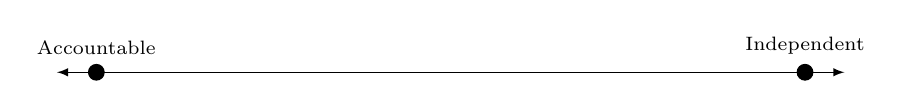
\begin{tikzpicture}
	% a straight line segment
	\draw[latex-latex] (-0.5,0) -- (9.5,0);
	%% the labels
	\node[fill=black,draw=black,circle,inner sep=2pt,label=above:{\scriptsize Independent}] at (9,0) {};
	\node[fill=black,draw=black,circle,inner sep=2pt,label=above:{\scriptsize Accountable}] at (0,0) {};
	\end{tikzpicture}
\end{figure}

Judicial independence takes two forms: \textit{de jure} and \textit{de facto} \citep{Feld2003,Rios2014, Rosenberg1991,Voeten2008}.  \textit{De facto} judicial independence reflects two concepts: first, a judge is independent when her decisions reflect her preferences, and second, even if a court is totally independent ``that lacking financial or physical means of coercion, courts depend on the assistance of other political authorities to enforce their decisions'' \citep[4]{Rios2014}. Can a judge with a set term of office reasonably expect to remain in office no matter which way they rule on a particular case? If the answer to that question is yes, the judge enjoys \textit{de facto} independence. 

\citet[3]{Rios2014} define \textit{de jure} judicial independence as ``formal rules designed to insulate judges from undue pressure, either from outside the judiciary or within.''  These are the institutional protections that allow a judge to be independent from the executive, public, legislature, or superior courts.  Examples of these protections include selection and retention methods, term lengths, and docket control.

Judicial independence itself is a latent concept, meaning that is cannot be measured directly \citep[203]{Treier2008}.  However, there exist indicators that allow us to measure both \textit{de jure} and \textit{de facto} judicial independence.  As \citet[5]{Rios2014} note, the indicators used to measure \textit{de jure} independence are easily observable, however, measuring the latent variable of independence is what is far more challenging.  Judicial independence is not a new concept, it has been examined for many years.  Owing to the latency of the concept, it has proven routinely difficult to measure.  The difficulty lies in identifying indicators that can assist us in the measurement.  Many of the existing studies share a common theme in the indicators that they use to determine \textit{de jure} judicial independence.  

\subsection*{Previous Studies}%Who's done it and why did their's suck
Existing efforts to operationalize de facto judicial independence have taken on a wide variety of forms. This is unsurprising, as most such measures were developed with specific research goals in mind, and are thus designed to capture particular aspects of independence that were of particular relevance to the study in question. At the same time, all share some common characteristics. First, all such measures are predominantly institutional in nature, in that they rely primarily on characteristics of the judicial institutions themselves as indicators of independence or lack thereof. Second, nearly all are observational (as opposed to interview-or survey-based) and rely on aggregation of varying numbers of partial indicators into a 
summary scale. Finally, all were developed for the cross-national context. The latter point is important, since indicators appropriate to a cross-national measure may or may not be similarly valid in the context of the U.S. states (and vice-versa).

\citet{Choi2010} develop a theoretical model of judicial independence in the form of a principal-agent relationship.  One of the key concepts of independence in this relationship is the identity of the principal.  In this case, the court as a whole but also individual judges act as the agent, and the appointing authority acts as the principal.  As \citeauthor{Choi2010} note, independence hinges on who is responsible for the initial appointment but also on who holds the power of reappointment.  As the number of principals increases, so does the amount of those who must be satisfied in order for the judge to maintain their position.  This principal-agent relationship is the basis for many of the assumptions in this model.  \citet{Choi2010}'s choice of indicators for judicial independence is entirely \textit{de facto} however.  \citet[296]{Choi2010} puts forth a hypothesis based on a collective-action problem.  When judges are elected by the public at large, instead of a single principal, there is instead an exponentially larger number, increasing the free-rider problem.  By contrast, in appointed states, with a single governor as the principal, there is no free-rider problem.  This is only marginally increased when using a commission based system, and is perhaps even attenuated by the lack of other political considerations of the committee as opposed to the governor.  However, in all commission system states, the governor is ultimately responsible for appointing the judges in question.  For example, their primary indicator for judicial independence is a ratio of the number of times that a judge writes an opinion that disagrees with their co-partisans.

\citet{Schmidhauser1987} develops an eleven part framework for a legal system based on neo-Weberian concepts.  Some of the components of this framework are: the concept that judicial institutions are based upon constitutional rather than ordinary statutory authority \citep{Schmidhauser1987}.  Judges are constitutionally protected with life tenure, and full establishment and acceptance of judicial review \citep[46-47]{Schmidhauser1987}.  The American states have accepted some of these concepts but clearly not all.  The American states are a mix of selection methods and tenure.  Many of the other indicators used in previous study, such as constitutional interpretation and judicial review, do not have any variation in the American context and are constitutionally protected in most state constitutions. 

Table \ref{otherindicators} shows a comparison of previous studies of \textit{de jure} judicial independence.  \citet{Rios2014} examine three measures of \textit{de jure} judicial independence: \citet{Feld2003}, \citet{Keith2002a}, and \citet{Laporta2004}.  In addition, they evaluate \citet{Apodaca2004} study.  Each of these studies develop a measure of \textit{de jure} judicial independence using different indicators and different methodologies.  Table \ref{otherindicators} shows the commonality of some of these measures such as appointment/retention methods and term lengths.  It also shows the lack of congruence in indicators of \textit{de jure} judicial independence shown in previous studies.

As \citet{Rios2014} note, there are some issues with the validity in each of these measures.  One main concern is that some of these measures are not directly related to independence.  Some of these measures are court accessibility, case allocation, right to strike, the four freedoms, pay comparisons, bans on torture, and legal origin \citep{Feld2003,Keith2002a,Laporta2004,Rios2014}.  The second concern is that in R\'{i}os-Figueroa and Staton's study many of the \textit{de jure} as well as many of the \textit{de facto} use indicators that capture both \textit{de jure} and \textit{de facto} independence.  \citealt{Laporta2004} attempt to measure \textit{de facto} independence by using \textit{de jure} independence as a proxy.  However, this is complicated by the fact that even though the institutional arrangements that derive \textit{de jure} independence are observable, \textit{de jure} independence itself is still a latent concept. 

\newgeometry{bottom=.5in}
\begin{landscape}
	\begin{table}[tb]\centering\caption{Comparision of Indicators of \textit{De Jure} Judicial Independence}\label{otherindicators}\small
		\begin{tabular}{rccccc}\hline
			Indicators	&	\citet{Feld2003}	&	\citet{Keith2002a}	&	\citet{Laporta2004}	&	\citet{Rios2006}	&	\citet{Melton2014}	\\\hline
			Anchored in the Constitution	&	X	&		&		&		&		\\
			Amendment Difficulty	&	X	&		&		&		&		\\
			Appointment Procedure	&	X	&		&	X	&	X	&	X	\\
			Tenure	&	X	&		&	X	&	X	&	X	\\
			Renewable Terms	&	X	&		&		&		&		\\
			Salary Insulation	&	X	&		&		&	X	&	X	\\
			Pay Comparison	&	X	&		&		&		&		\\
			Court Accessibility	&	X	&		&		&		&		\\
			Case Allocation	&	X	&		&		&		&		\\
			Constitutional Interpretation	&	X	&		&	X	&	X	&		\\
			Published Decisions	&	X	&		&		&		&		\\
			Four Freedoms	&		&	X	&		&		&		\\
			Right to Strike	&		&	X	&		&		&		\\
			Writ of \textit{Habeas Corpus}	&		&	X	&		&		&		\\
			Public Trial	&		&	X	&		&		&		\\
			Fair Trial	&		&	X	&		&		&		\\
			Ban on Torture	&		&	X	&		&		&		\\
			Case Law	&		&		&	X	&		&		\\
			Legal Origin	&		&		&	X	&		&		\\
			Number of Courts	&		&		&		&	X	&		\\
			Number of Judges	&		&		&		&	X	&		\\
			Budget Control	&		&		&		&	X	&		\\
			Impeachment	&		&		&		&	X	&	X	\\
			Promotions	&		&		&		&	X	&		\\
			Transfers	&		&		&		&	X	&		\\
			Sanctions	&		&		&		&	X	&		\\
			Statement of Judicial Independence	&		&		&		&		&	X	\\\hline
		\end{tabular}
	\end{table}
\end{landscape}
\restoregeometry

\doublespacing\normalsize
\citet*{Melton2014} create an additive index that uses six aspects of judicial independence.  This model as well as that of \citet*{Feld2003} and \citet*{Keith2002b} use an additive index.  Table \ref{otherindicators} shows previous studies of \textit{de jure} judicial independence and the indicators that were used.  These previous studies show the wide variation in indicators used, as well as the most basic method of creating a measure.  Only two of these measures, appointment procedure and tenure, are used in more than three of the five studies shown.

Many of the previous studies of latent variables were constructed using additive models.  The most widely cited use of this in comparative politics is POLITY IV \citep{Polity}.  This has also dominated the study of judicial independence.  Most if not all previous studies use additive indices \citep{Feld2003,Keith2002a,Laporta2004} and some still continue to do so today \citep{Melton2014}.  Following work in other areas more recent work has adopted an IRT approach \citep{Martin2002,Treier2008,Schnakenberg2014,Linzer2014,Fariss2014}.

As \citet{Linzer2014} show, a  properly specified Bayesian IRT model can be more informative.  The most important benefit of using this type of model is that there is no assumption made about the space between the cut points of each level of indicator, and between the indicators themselves \citep{Jackman2008,Schnakenberg2014}.  This method provides important tools in model specification and diagnostics that are lost when using an additive model.  Many of the potential indicators of \textit{de jure} judicial independence are dichotomous or nominal, having no ordering, and at best they are ordinal, as in the case of selection methods.  Only the length of tenure is clearly ordered in that longer terms indicate independence as opposed to shorter terms.  Other indicators such as selection, retention, and control of the docket, while theoretically grounded do not easily lend themselves to additive models.

Take the example of selection method, when using an additive scale the difference between a partisan and non-partisan election are considered to be a one unit increase along the latent trait of judicial independence, whereas that same increase of one unit can be considered between the change from a non-partisan election to a legislative appointment.  In this case there are vastly fewer people involved in the selection process between these two, reducing the amount of campaign funds needed.  The same example can be used between the levels of term length.  When moving from a short term, say 1-3 years, to 4-6 years is not the same as moving from a ten year term to a lifetime or quasi-lifetime term.

\citet*{Linzer2014} create a measurement model that exclusively models \textit{de facto} judicial independence.  The measurement model created below is a complimentary addition to that created by \citeauthor{Linzer2014}.  This model focuses exclusively on \textit{de jure} judicial independence, but uses a similar statistical model to that of \citeauthor{Linzer2014}.  

\section{Indicators}\label{Indicators}
As shown in Table \ref{otherindicators} the most commonly employed indicators in previous studies of \textit{de jure} judicial independence are appointment procedure and tenure.  Each author codes these slightly differently however, \citet{Feld2003} use an ordinal scale for term tenure, while \citet{Melton2014} use a dichotomous variable for lifetime terms.  The same is true for appointment procedures.  In addition, most previous studies were cross-national and do not allow for the various forms of elections that occur under the American system.    

\begin{figure}[tbh]\centering\caption{Selection Method Independence Continuum}\label{selectioncontinuum}
	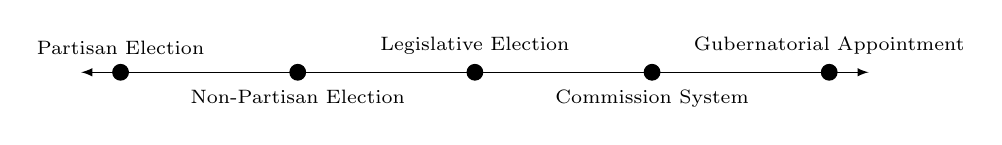
\begin{tikzpicture}
	% a straight line segment
	\draw[latex-latex] (-0.5,0) -- (9.5,0);
	%% the labels
	\node[fill=black,draw=black,circle,inner sep=2pt,label=above:{\scriptsize Gubernatorial Appointment}] at (9,0) {};
	\node[fill=black,draw=black,circle,inner
	sep=2pt,label=below:{\scriptsize Commission System}] at (6.75,0) {};
	\node[fill=black,draw=black,circle,inner
	sep=2pt,label=above:{\scriptsize Legislative Election}] at (4.5,0) {};
	\node[fill=black,draw=black,circle,inner
	sep=2pt,label=below:{\scriptsize Non-Partisan Election}] at (2.25,0) {};
	\node[fill=black,draw=black,circle,inner sep=2pt,label=above:{\scriptsize Partisan Election}] at (0,0) {};
	\end{tikzpicture}
\end{figure} 

\subsection*{Selection Method}
The method of judicial selection is probably the most important variable in determining judicial independence. There are five primary selection methods in use in the United States: executive appointment, legislative appointment, merit selection, non-partisan election, and partisan election. Some states use a mix of these methods; Michigan and Ohio for example, both employ systems which blend partisan primaries with nonpartisan general elections.\footnote{Following normal practice in this field, these states are coded as non-partisan \citep{Canes-Wrone2012, Caldarone2009}, however Tiede \citeyearpar{Tiede2006} does the opposite and codes them as partisan states. Nelson, Caufield, and Martin \citeyearpar{Nelson2013} discuss this coding decision at length.  In accordance with recommendations made in their article, this model will be conducted both ways and examined for differences, with theoretical justifications for both methods made clear.}    Under \citet{Hall2007}'s theory of judicial accountability, I consider executive and legislative appointments to be the most independent/least accountable of the selection methods.  For the majority of states, executive appointment was the original method of appointment.  \footnote{In all executive and legislative appointment states, the Governor is the final appointing authority.  In all executive and legislative appointment states, judges require a confirmation vote of one or both houses of the state legislature.}  Figure \ref{selectioncontinuum} shows how these methods map on to a single dimension continuum with the most accountable method on the left and the most independent method on the right. 

\begin{figure}[tbh]\centering\caption{Current Judicial Selection Methods}\label{selectionmap}
	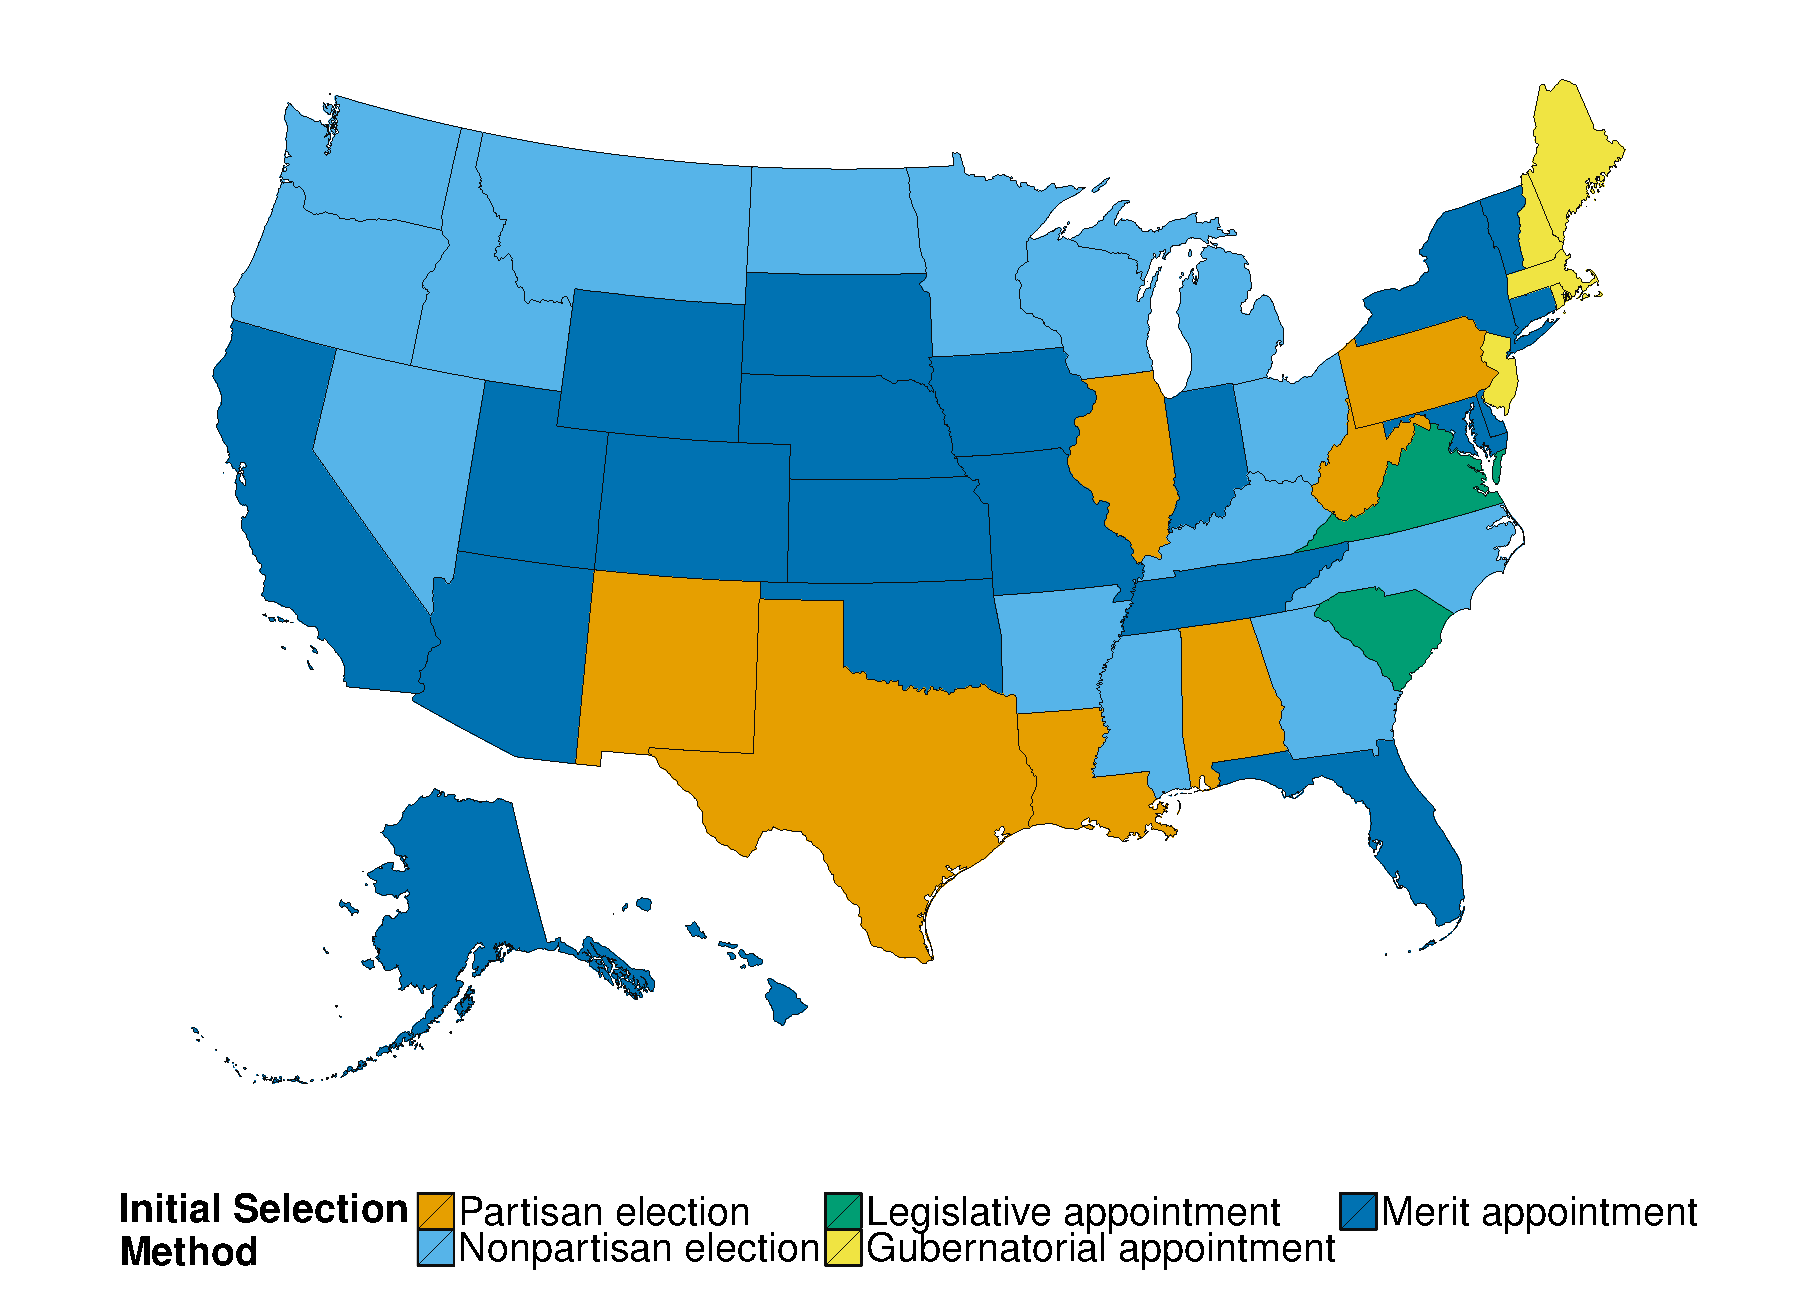
\includegraphics[scale=.5]{graphics/colr_select.pdf}
\end{figure}

The second type of selection system is the Commission System or “merit selection.” The commission system plan came about with the adoption of the Missouri Nonpartisan Court Plan in 1940 \citep{Watson1969}. This system was created with the goal of removing partisanship in judicial selection. This system created a judicial nominating commission who reviews applications and interviews candidates judicial posts. The commission consists of three lawyers selected by the Missouri Bar Association, and three citizens selected by the governor as well as the Chief Justice of the Missouri Supreme Court who serves as the chair of the commission. When a vacancy exists in the courts, the commission submits three names to the Governor who then selects one nominee which is confirmed by the State Senate. Once the judge has completed at least one year in office they stand for retention election. Retention elections are on separate ballots and only ask the voter to vote whether the judge should be retained. This description of the Missouri Plan is representative of the other twenty states which use similar systems.  There is no partisan affiliation listed on the ballot \citep{Watson1969}.  The most substantive difference between commission systems and other systems is the attempt to remove partisanship completely. Appointment, as well as partisan elections, are both acknowledged to be partisan acts, while proponents of commission systems and non-partisan elections claim that these systems eliminate partisanship from judicial selection. 

There are two types of electoral selection: partisan and non-partisan.  Electoral systems are considered to be the least independent due to the number of actors involved in the selection process \citep{Choi2010}. These judges are also generally forced to raise money for advertising and other campaign related expenses.  Debate exists about the ethical implications of raising this money from businesses, interest groups, and litigators that may appear before these judges.\footnote{For empirical evidence of this see \citep{Gibson2008}.}  Elected judges are selected by the electorate in statewide elections.  \citet{Caldarone2009} puts forth the view that when electing judges, the public will elect the judges that most closely match their own personal preferences.  However \citet{Debow2013} states that ``non-partisan judicial elections do not compare favorably with partisan judicial elections'' because the former inhibit the voters ability to make informed decisions.

\subsection*{Retention Method}
Creation of retention elections were a hallmark of the merit selection plan created in Missouri. Retention elections differ from partisan and non-partisan elections in that there is only one candidate involved in the election. As \citeauthor{Reid1999} summarizes: \begin{quote}``Judicial retention elections are intended to preserve the court’s role as an impartial and detached resolver of disputes by ensuring that judges can retain their seats without engaging in the fund raising, politicking, and electioneering that characterize political elections and the political process,'' \citep[68]{Reid1999}.\end{quote}  Retention elections simply ask voters to approve or disapprove of the judge in office. Ballots questions usually appear in the form of: ``Shall each of the persons listed be retained in office as Judge of the Appellate Court, First Judicial District?''

All but the four states which have life or quasi-life terms employ some manner of retention elections. Some states use retention elections such as those listed above. Others use the same type of partisan or non-partisan election as they use for their initial selection. No state uses a commission system then requires the judge to run in a contested election.\footnote{The exception to this is in the case of a judicial vacancy.  If a judge resigns, or dies in office, states have selection mechanisms in place that can differ from the official selection system.  For example, in the case of New Mexico ``All judicial vacancies are filled by the governor from a list of candidates recommended by a judicial nominating commission. The appointee must then compete in a partisan election at the next general election to serve the remainder of the unexpired term'' \citep{AJS}.}  Also no states utilizes a partisan election for initial selection and then uses non-partisan elections for retention.  Contested elections, whether partisan or non-partisan, are considered to be the least independent \citep{Choi2010,ABA2003,Canes-Wrone2012}. Judges who do not face any electoral accountability are considered the most independent in this context.

\begin{figure}[tbh]\centering\caption{Retention Method Independence Continuum}\label{retentioncontinuum}
	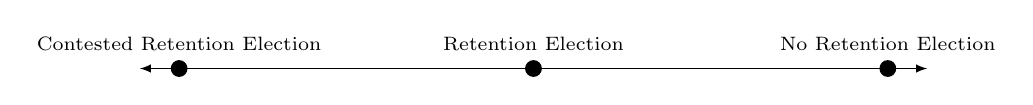
\begin{tikzpicture}
	% a straight line segment
	\draw[latex-latex] (-0.5,0) -- (9.5,0);
	%% the labels
	\node[fill=black,draw=black,circle,inner sep=2pt,label=above:{\scriptsize No Retention Election}] at (9,0) {};
	\node[fill=black,draw=black,circle,inner
	sep=2pt, label=above:{\scriptsize Retention Election}] at (4.5,0) {};
	\node[fill=black,draw=black,circle,inner sep=2pt,label=above:{\scriptsize Contested Retention Election}] at (0,0) {};
	\end{tikzpicture}
\end{figure}

Retention elections are admittedly only a matter of degrees more or less independent than contested elections. Figure \ref{retentioncontinuum} shows how methods of retention can map on to the judicial Independence Continuum.  There is still some debate on whether retention elections create a more independent judiciary. The ABA defends its position that retention elections are more independent and recommends them for all states that utilize elections to retain judges \citep{ABA2003}.  \citep{Canes-Wrone2012} take a divergent position and posit that judges are susceptible to losing their seats based on only one or two salient decisions and also susceptible to attacks from single-issue groups.  This occurred in 2010 when three justices on the Iowa Supreme Court were ousted. These justices had voted to strike down Iowa’s ban on same-sex marriage. There was a prolonged campaign by single-issue groups opposed to same-sex marriage resulting in the judges removal \citep{Iowa2010}.

\subsection*{Term Lengths}
The length of a judicial term is another important factor in determining the level of judicial independence.  In many commission system states seats are vacated by either promotion, retirement, or death. Replacement judges are then appointed to fill out the unexpired terms. The initial term lengths for the new judges in those states range from appointment until the next general election, or from appointment through the remainder of the full term. Subsequent term length is the length of the terms after the initial term. For most elective states this is the same as the initial term length, and for retention states, this the length of a standard term. Term lengths for initial terms range from one year to fourteen years\footnote{While there are four states which have lifetime or quasi-lifetime (age limited terms) only New Jersey requires reappointment after an initial term.} while subsequent terms range from six years to lifetime terms.\footnote{Many states also have statutory term lengths also utilize a mandatory retirement age.}  These term lengths can be compared to U.S. House of Representatives terms which are two years, and U.S. Senate terms which are six years.  The longer that a term is, the more independent choices a judge can make before being held accountable prior to an election.  Figure \ref{termcontinuum} shows how varying term lengths map on to the Independence Continuum.  According to \citet[31]{Rios2006} ``terms must be long enough to reduce the vulnerability of Supreme Court judges.  Tenure need not be for life, but if it coincides with that of appointing authorities then there is the potential for abuse.''\footnote{\citet{Rios2006} uses a binary coding scheme in his study, coding a term length as independent if it was longer than the appointing authority.}  As Hall and others show, most of strategic voting of judges is done in the year prior to an election \citep{Hall1987,Hall1985,Brace2008,Canes-Wrone2012}.  

\begin{figure}[tbh]\centering\caption{Term Length Independence Continuum}\label{termcontinuum}
	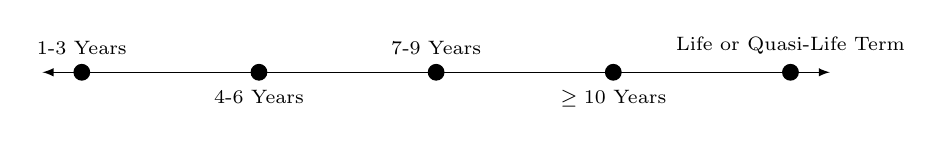
\begin{tikzpicture}
	% a straight line segment
	\draw[latex-latex] (-0.5,0) -- (9.5,0);
	%% the labels
	\node[fill=black,draw=black,circle,inner sep=2pt,label=above:{\scriptsize Life or Quasi-Life Term}] at (9,0) {};
	\node[fill=black,draw=black,circle,inner
	sep=2pt,label=below:{\scriptsize $\geq10$ Years}] at (6.75,0) {};
	\node[fill=black,draw=black,circle,inner
	sep=2pt,label=above:{\scriptsize 7-9 Years}] at (4.5,0) {};
	\node[fill=black,draw=black,circle,inner
	sep=2pt,label=below:{\scriptsize 4-6 Years}] at (2.25,0) {};
	\node[fill=black,draw=black,circle,inner sep=2pt,label=above:{\scriptsize 1-3 Years}] at (0,0) {};
	\end{tikzpicture}	
\end{figure}

There are several arguments for the inclusion of term length as an indicator of judicial independence. The ABA views the term length question as a matter of experience in that lawyers who are experienced and qualified will be reluctant to leave successful private practices if they are forced to return to the job market after only a few years \citep[97]{ABA2003}.   The argument against longer terms is that longer terms provide less opportunity for accountability. The ABA recommends an actively enforced judicial discipline system, which will ensure accountability for systems that do not rely on re-selection stating that judges should only be removed for ``cause'' \citep[103]{ABA2003}.\footnote{This is in reference to an ethical or criminal violation, rather than a punitive punishment as the result of an opinion.  The clearest example of this would be the Iowa case where judges were ousted based on an ideological view, rather than as a breach of ethics or the law.}  The low level of judicial turnover disputes this point of view. In 2012, only 6 of the judges on state supreme courts were not retained. For the years 1964-1998, there were 4,588 retention elections with only 52 judges being voted out of office \citep{Aspin2000}.  

There are several arguments for a connection between longer term lengths and increased judicial independence as well as alternatives such as limiting judges to only a single term. A single term would obviate the need for reappointment or campaigning for their next term \citep{Carrington1998}.  Former Presiding Judge of the Texas Court of Criminal Appeals Morris Overstreet has stated ``if you don't have to go back and face the voters, you don't have to worry about how they're going to retaliate or if they're going to retaliate'' \citep{ABA2003}.  This has the drawback of returning judges to private practice, which may have an effect on their decisions made while on the bench.  No state currently has adopted this practice.

\citet{Hall1987a}'s study of the Louisiana Supreme Court shows that when faced with electoral accountability, the judges have a tendency to avoid casting votes on unpopular issues. Hall concludes that this system ``does not present the opportunity for the unfettered exercise of individual preferences'' \citep[46]{Hall1987a}.  Hall also concludes that justices who perceive themselves to have views inconsistent with public opinion,  and who desire to keep their jobs, may be hesitant to publish opinions which are against public opinion. Hall states that ``whether voters and opponents are cognizant of the justices’ behavior or not, certain justices seem to fear the prospect of electoral sanction and consequently alter their behavior'' \citep[1123]{Hall1987b}.  While voters’ knowledge of justices' records is questionable, certainly the judges' actions are not.  As Hall shows, judges act as if voter's will have knowledge of their records and vote strategically to minimize the electoral losses they may suffer.

\subsection*{Docket Control}
The ability of a court to control its own docket is another important factor in examining \textit{de jure} independence.  Docket control comes in many forms, ranging from complete discretionary control, as in the case of the U.S. Supreme Court, which can grant or deny any appellate case that it wishes to hear with few exceptions, to states such as Wyoming which have no intermediate appellate courts, and therefore has very little control over its appellate docket. There are also many states which have mandatory appeals on certain subject matter or litigants, and discretionary appeals on other types of cases.  Typically, docket control is set through statues passed by the state legislature, similar to the appellate jurisdiction of the U.S. Supreme Court, although some states have their docket discretion set through the state constitution.\footnote{Death penalty cases are an exception to this general rule.  In many cases death penalty appeals must be heard by the Court of Last Resort for that state, and this reduces the court's discretion in these cases.  In the case of this analysis, this exception will be ignored.  For states which utilize complete discretionary docket control except for death penalty cases, they will be coded as having complete discretion.}

\begin{figure}[tbh]\centering\caption{Docket Control Independence Continuum}\label{docketcontinuum}
	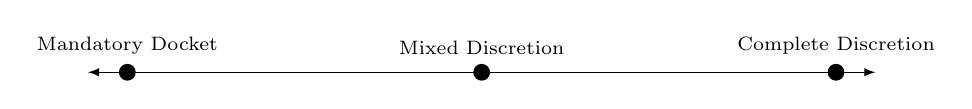
\begin{tikzpicture}
	% a straight line segment
	\draw[latex-latex] (-0.5,0) -- (9.5,0);
	%% the labels
	\node[fill=black,draw=black,circle,inner sep=2pt,label=above:{\scriptsize Complete Discretion}] at (9,0) {};
	\node[fill=black,draw=black,circle,inner
	sep=2pt,label=above:{\scriptsize Mixed Discretion}] at (4.5,0) {};
	\node[fill=black,draw=black,circle,inner sep=2pt,label=above:{\scriptsize Mandatory Docket}] at (0,0) {};
	\end{tikzpicture}
\end{figure}

The ability of a court to control its docket has multiple facets to it's effect on independence.  The first is that if a court has control over its docket, then the workload of the court can be reduced to only those cases that the court wishes to make a statement on, rather than hearing every case, including those on which there is already clear precedent \citep{Maltzman2000}.  Also, reduced workload enables a court to spend more time on those cases that it deems important.  While this may seem more related to efficiency than independence, the two are inter-connected in this case.  As Squire notes, the ability to pick and choose cases allows an appellate court to craft their decisions more carefully than a court which has no discretion \citep{Squire2008}.

The second aspect of docket control on judicial independence stems directly from the first.  Not only can judges spend more time on cases under a discretionary docket, but they can pick and choose the cases that they want to issue an opinion on.  As Fontana notes, this can be very important to both the influence and the legitimacy of a court \citep{Fontana2011}.  Fontana notes that had the \textit{Brown v. Board of Education} decision been decided ten years earlier, it might not have had the effect that it had, due to a lack of support from the President, and antipathy from southern states, and their representatives in Congress.  This is supported by \citet{Rosenberg1991} in light of the very extensive process to bring the country in to compliance with the Court's ruling in \textit{Brown}.  Had this process happened earlier, there might have been no compliance, causing both extended oppression of African-Americans in the South, as well as a severe blow to the legitimacy of the Court.  Fontana refers to this as ``legitimacy timing'' \citep[627]{Fontana2011}.  

Another important aspect of docket control is the effect that it has on a judge's voting preferences.  Whether following a strictly legal interpretation, or an ideological preferences, a key part of judicial independence is a judge's ability to vote her preferences.  \citeauthor{Songer2003} note that when courts have discretionary control over their dockets, the judges are much more likely to follow the attitudinal model of voting preferences \citep{Songer2003}.  This would lead us to believe that discretionary control allows more freedom in the preferences that judges exercise in this case.   This is also supported by Melinda Gann Hall's study of the Louisiana Supreme Court.  Hall finds that in discretionary cases, there is a significant number of dissents, rather than in mandatory cases, which shows much more unanimous decisions \citep{Hall1985}.  There are several hypotheses for this outcome, chiefly that under mandatory review, there are many more ``easy'' cases.  That is cases which have a clear precedent and had no complex legal complications.  These cases could have been successfully disposed of by the lower courts, but were required to be heard by the state supreme court.   

The most important aspect of a court's jurisdictional control comes from their independence from the executive and legislature.  This is especially a concern when the government is a party to a case that the court could potentially hear.  As \citet[6]{Rios2014} note, ``Indeed, a court that offers little constraint on government can appear to be highly constraining if it chooses its cases wisely. It certainly can ensure systematic compliance, which makes inferring judicial influence from the outcomes of legal conflicts difficult.''  They also posit that judicial decision making can appear to be independent if the court removes contentious cases from its docket.  The example of same-sex marriage can illustrate this quite clearly.  Had the Iowa Supreme Court simply chosen to uphold the lower court ruling in \cite{iowagay}, they most likely could have avoided the lengthy campaign that was mounted against the retention of three justices that ultimately resulted in their dismissal.

\section{Methodology}\label{Methods}
\subsection*{Data}
The model uses institutional data on the courts of last resort used by the 50 states in the United States.  There are 52 courts of last resort in the United States.\footnote{The court of last resort for the District of Columbia is the District of Columbia Court of Appeals.  As the District of Columbia is not a state and its courts fall under the federal system, it is omitted in this study.  The D.C. Superior Court is the trial court and refers all appeals to the D.C. Court of Appeals.  Its judges are appointed by the President and confirmed by the Senate to fifteen year terms.}  Each state has a court while Texas and Oklahoma have specialized courts for civil and criminal.  In this study these court systems will be examined together as they have identical institutional arrangements.  

I create three models of \textit{de jure} judicial independence.  The first uses the first four indicators discussed below.  This model comprises the 50 states from 1800-2012.  The second model uses five indicators, with the addition of a docket control indicators from 1800-2012.  The reason for the two different models is the lack of available data on docket control prior to 1970.  The states had a variety of control over their dockets from 1970 through the present.  However, between 1940 and 1970 the data is nearly non-existent due to a lack of reliable surveys of state court organizations.  The post-1970 data was provided by the Bureau of Justice Statistics (BJS) and the National Center for State Courts (NCSC) \citep{BJS1993,BJS1998,BJS2004}.  

The third model specification is a regime change model, which only includes only state-year observations that indicate a change in any of the four indicators used in the primary specification.  

Prior to 1940, in addition to the data being non-existent, there was also much dispersion in the interpretation of docket control based on the individual states.  In many of these states, even if there was an ``appeal by right,'' some states interpreted this as mandatory jurisdiction, while others did not.  These discrepancies lead toward a more \textit{de facto} indicator than is being addressed in this paper.  With the standardized definitions used in the BJS and NCSC reports, it becomes useful to add this indicator in for a post-1970 model, but as shown below, the wider variance in selection/retention methods and term lengths, still make a study of a longer time span useful, despite the lack of jurisdictional control data.  

\subsection*{Indicators}
All of the indicators are ordinal variables with 0 representing the most independent moving towards least independent.  \texttt{APPT} is coded from 0-4, which is the appointment method that is used for a judge's initial appointment.  \texttt{TERM1} is coded from 0-3 and represents the length of the judge's initial term.  \texttt{TERM2} is coded in a similar manner as \texttt{TERM1} and represents the length of the judge's subsequent terms after their first retention or reappointment. 
%-------------------------------------------------------------
\begin{table}[!htb]\singlespacing\centering
	\caption{List of Indicators}\label{Indicators}
	
	\begin{tabular}{ccl}\hline
		\textbf{Variable}	&		&	\textbf{Code}	\\\hline\hline
		APPT	&		&	Appointment Method	\\
		0	&	-	&	Gubernatorial Appointment	\\
		1	&	-	&	Commission System	\\
		2	&	-	&	Legislative Appointment	\\
		3	&	-	&	Non-Partisan Election	\\
		4	&	-	&	Partisan Election	\\\hline
		TERM1	&		&	Initial Term Length	\\
		0	&	-	&	Lifetime or Quasi-Lifetime Term\\
		1	&	-	&	$\geq10$ Years	\\
		2	&	-	&	7-9 Years	\\
		3	&	-	&	4-6 Years	\\
		4	&	-	&	1-3 Years	\\\hline
		TERM2	&		&	Subsequent Term Length	\\
		0	&	-	&	Lifetime Term	\\
		1   &   -   &   $\geq10$ Years \\
		2	&	-	&	7-9 Years	\\
		3	&	-	&	4-6 Years	\\
		4	&	-	&	1-3 Years	\\\hline
		RETELE	&		&	Method of Retention	\\
		0	&	-	&	No Retention Election	\\
		1	&	-	&	Retention Election	\\
		2	&	-	&	Contested Retention Election	\\\hline
		DOCKET	&		&	Docket Control Discretion	\\
		0	&	-	&	Complete Discretion	\\
		1	&	-	&	Mixed Discretion	\\
		2	&	-	&	Mandatory Docket	\\\hline
	\end{tabular}
	
\end{table}
%--------------------------------------------------------------
There is one major difference however, in that 0 represents those states in which the judge is initially appointed to a lifetime term\footnote{The only major time this is an issue is in New Jersey, in which judges are initially appointed to a seven year term and then reappointed to a lifetime term.  However, since New Jersey is represented with a seven year term initially, this is different than if they were initially appointed to a lifetime term and therefore their subsequent term is greater than ten years.}.  In many states, these two terms are identical.  These differences are primarily in merit selection states which have one to three year terms followed by a retention election and then have longer terms after the first retention election.  Coding term lengths as ordinal rather than continuous, allows for consistent interpretation across the model.  \texttt{RETELE} is coded from 0-2 and indicates the method of retention.  0 indicates a simple reappointment procedure with no election.  1 represents an uncontested retention election, most common under the merit selection system, but also used in states that utilize partisan or non-partisan election systems.  2 indicates a contested retention election, either partisan or non-partisan.  \texttt{DOCKET} represents the amount of discretion that a court has over its docket.  0 is a completely discretionary docket, while 2 is no discretion.  A 1 indicates a mix of discretionary and mandatory appeals. Table \ref{Indicators} shows the coding for all levels of each indicator. 

\section{Model}\label{Model}
The model used for this is a Bayesian Dynamic-Ordinal Item Response Theory Model.  This model is the same as that developed by \citet{Schnakenberg2014}.  Rather than examining countries' respect for human rights, this model examines the level of \textit{de jure} judicial independence that a state's judicial institutions represents. \footnote{There is also one major difference in that \citeauthor{Schnakenberg2014} measure a \textit{de facto} level of respect for human rights, in that they look at actual numbers of torture, extra-judicial killings, and disappearances in a given year, I am looking at institutional arrangements, which typically has much less within-state variance from year to year.}	

I assume that the observed indicators for each state-year are functions of a single dimensional latent variable (the Judicial Independence Continuum) that represents the level of \textit{de jure} judicial independence.  For each state-year observation, let $i$ index the state and $t$ index the year.  or each model, there are $J$ indicators $J=1$,...,$J$ each of which is ordinal.\footnote{For definitions of each level of indicators, see Table \ref{Indicators}} I estimate each $\theta_{it}$, which is the latent level of \textit{de jure} judicial independence of each state $i$ in year $t$ \citep[7]{Schnakenberg2014}.

Let $i=1$,...,$N$ index cross-sectional units and $t=1$,...,$T$ index time periods.  In each time, period, I observe values $y_{ij}$ for each of $j=1$,...,$J$ indicators for each unit.  Each indicator is assumed to be ordinal and can take on $K_j$ values.\footnote{For term length indicators, these have been collapsed into five ordered categories.  This is due to the relative infinite value of a life or quasi-life term.  A previous specification of this model was considered using the average length of term in office for each justice that had served on the court under the life or quasi-life term.  This specification was rejected as introducing a questionable degree of \textit{de facto} independence into what is a purely \textit{de jure} measurement model.}  The responses to each of the items depend on a single latent variable $\theta_{it}$, which may vary across units and over time. I assume that all indicators are independently drawn from a logistic distribution \citep[7]{Schnakenberg2014}. 

For each indicator, there is an item discrimination parameter $\beta_j$ and a set of $Kj-1$ difficult cut-points.\footnote{For more detail on these cut-points see \citep{Treier2008,Schnakenberg2014}.  } \citep[7]{Schnakenberg2014}.  A benefit of using institutional arrangements, which are observable with readily available data is that any error that is introduced into the indicators is the result of coding errors rather than perceptional errors found in survey responses.  

The probability distribution for a given response to item $j$ is observed as:
\begin{align}
P[y_{ij}=k]=F(\alpha_{jk}-\theta_{it}\beta_j)-F(\alpha_{jk-1}-\theta_{it}\beta_j)
\end{align} $F(\cdot)$ is the logistic cumulative distribution function.  I assume the local independence of responses across units, the likelihood function for $\beta$, $\alpha$, and $\theta$ given the data is\footnote{For a more detailed explanation of the assumptions made in this likelihood, see \citep[8]{Schnakenberg2014}.}:
\begin{align}\label{like}
{\cal L} (\beta,\alpha,\theta|y)=\prod_{i=1}^{N}\prod_{t=1}^{T}\prod_{j=1}^{J}[F(\alpha_{jy_{itj}}-\theta_{it}\beta_j)-F(\alpha_{jy_{itj}-1}-\theta_{it}\beta_j)]
\end{align} 

If $\theta$, (\textit{de jure} judicial independence), was able to be observed, the likelihood function shown in Equation \ref{like} would be equivalent to an independent ordinal logistic regression model \citep[8]{Schnakenberg2014}.  There are three basic independence assumptions considered for IRT models.  The assumptions are: (1) local independence of different indicators within the same state -- year, (2) local independence of indicators across states within years and (3) local independence of indicators across years within states \citep[8]{Schnakenberg2014}.  The implication of this is that each $y_{itj}$ are independently drawn conditional on $\theta$.  The only relationship between two item responses is that they are both measure the same latent variable, $\theta$. \citet[8]{Schnakenberg2014} discuss the assumptions made in this model in greater detail.  I relax Assumption 1 slightly in that there is some correlation between selection retention methods. For example, there are no states which use a commission system for initial selection and then require judges to run in competitive elections.\footnote{This assumption does not extend to filling judicial vacancies.  For example, New Mexico uses a merit selection system to fill judicial vacancies and then requires the incumbent to run in a competitive partisan election at the next general election \citep{AJS}.  I consider this to be an artifact of the \textit{de facto} nature rather a factor of \textit{de jure} judicial institutions.}  However, their Assumption 3, is a matter of concern in this model for the same reason as \citep{Schnakenberg2014}.  Assumption 3 relates to the local independence of indicators across years within states \citep[8]{Schnakenberg2014}.  Rather than attempting to measure a regime's respect for human rights as in \citet{Schnakenberg2014}, I am measuring an institutional arrangement by each state.  In each state there is a yearly potential to change selection methods, keeping intact a relaxed version of this assumption.  This relaxation of Assumption 3 comes from the informative priors used by \citet[8]{Schnakenberg2014}.    

\section{Results}\label{Results}
\subfile{results.tex}

\section{Validation}\label{Validation}
\subfile{validation.tex}

\section{Application}\label{Application}
\subfile{application.tex}

\singlespacing
\bibliographystyle{apsr}
\bibliography{measurementbib}

\appendix
\section{Coding Notes}\label{CodingNotes}
\begin{itemize}
	\item Arkansas- In 1868, the Chief Justice was appointed by the Governor, with Senate Consent, with the Associate Justices elected by the people.  This is coded as partisan election since the majority of the justices are elected.
	
	\item Connecticut- from 1784 through 1818 Judges were appointed by the Legislature, but the tenure in office was dependent upon the action of the legislature.  These years are coded as missing and subsequently dropped from the dataset.
	
	\item Delaware- The original court of last resort was the Court of Appeals, and the data is coded as such.  The Supreme Court was created by constitutional amendment in 1951, at which point the data is coded to reflect the Supreme Court.
	
	\item Michigan- In 1939, a constitutional amendment passed calling for non-partisan elections for judges, except the Supreme Court, which would continue to be nominated at party conventions.  This is coded as a non-partisan following practice in this field.
	
	\item New Jersey- AJS Data does not reflect the Constitutional amendment in 1983, which extended subsequent terms to a term of good behavior.
	
	\item New Mexico- Judges are elected for the remainder of the unexpired term.  This could be up to 8 years, so it was coded as such.
	
	\item Oklahoma is examined individually, but both courts have mandatory jurisdiction.-2004
	
	\item Pennsylvania- From 1874 to 1968 Supreme Court justices were elected to twenty-one year terms and were not eligible for reelection.  This is coded as a 0 for the subsequent term.
	
	\item Tennessee- Constitution says qualified electors, however, by executive order the governor has created a nominating commission
	
	\item Texas is examined individually, SC has discretionary jurisdiction, but COA has mandatory in sentencing issues, so this is coded as mixed.- 2004
	
	\item Retention Elections- Gubernatorial reappointment, judicial commission reappointment, legislative reappointment are coded as No Retention Elections.
	
	\item Docket Control- This is established by looking at Criminal and Civil cases.  Administrative agency decisions are omitted, as well as death penalty cases.
	
	\item Docket Control- Observations between BJS reports are assumed to be static.
\end{itemize}

\section{Comparative Constitutions Project Variables}\label{CCPCode}
\begin{itemize}
	\item Statement of Judicial Independence -- \textbf{[JUDIND]} -- Does the constitution contain an explicit declaration regarding the independence of the central judicial organ(s)? 
	\item Life Term -- \textbf{[SUPTERM]} -- What is the maximum term length for judges for the highest ordinary court? 
	\item Selection Procedure -- \textbf{[SUPNOM,SUPAP]} -- Who is involved in the nomination of judges to the highest ordinary court? and Who is involved in the approval of nominations to the highest ordinary court? 
	\item Removal Procedures -- \textbf{[JREM, JREMPRO, JREMFIRP, JREMSECP, JREMBOTP, JREMAP]} -- Are there provisions for dismissing judges? and Who can propose the dismissal of judges? and Who can approve the dismissal of judges?
	\item Removal Conditions -- \textbf{[JREMCON]} -- Under what conditions can judges be dismissed?
	\item Salary Insulation -- \textbf{JUDSAL} -- Does the constitution explicitly state that judicial salaries are protected from governmental intervention?
\end{itemize}

\section{Ginsburg and Melton Replication Data}\label{GMData}
\begin{table}[!h]\centering\footnotesize
	\begin{tabular}{|r|ccc|r|ccc|}\hline
		State	&	Additive	&	IRT	&	G\&M	&	State	& Additive	&	IRT	&	G\&M	\\	\hline
		Alabama	&	12	&	-1.31091129	&	1	&	Montana	&	9	&	-0.581144339	&	1	\\	
		Alaska	&	5	&	0.368783882	&	4	&	Nebraska	&	9	&	-0.072441168	&	2	\\	
		Arizona	&	8	&	-0.012413602	&	4	&	Nevada	&	11	&	-0.909487793	&	3	\\	
		Arkansas	&	9	&	-0.578075634	&	3	&	New Hampshire	&	1	&	1.533583382	&	2	\\	
		California	&	3	&	0.673908309	&	4	&	New Jersey	&	2	&	1.768516335	&	3	\\	
		Colorado	&	7	&	0.384204611	&	3	&	New Mexico	&	10	&	-0.905869398	&	1	\\	
		Connecticut	&	5	&	0.760455328	&	3	&	New York	&	3	&	1.103325872	&	3	\\	
		Delaware	&	3	&	1.099737375	&	3	&	North Carolina	&	9	&	-0.576762507	&	3	\\	
		Florida	&	9	&	-0.076706106	&	3	&	North Dakota	&	7	&	-0.291201696	&	3	\\	
		Georgia	&	11	&	-0.908038872	&	2	&	Ohio	&	10	&	-0.89905174	&	3	\\	
		Hawaii	&	3	&	1.100137397	&	4	&	Oklahoma	&	9	&	-0.079603662	&	3	\\	
		Idaho	&	11	&	-0.913301035	&	1	&	Oregon	&	11	&	-0.903450105	&	1	\\	
		Illinois	&	7	&	0.16588657	&	3	&	Pennsylvania	&	7	&	0.169291474	&	3	\\	
		Indiana	&	7	&	0.387192126	&	4	&	Rhode Island	&	1	&	1.520687113	&	5	\\	
		Iowa	&	8	&	0.155611872	&	4	&	South Carolina	&	4	&	0.900738263	&	4	\\	
		Kansas	&	9	&	-0.079342362	&	4	&	South Dakota	&	8	&	0.145693754	&	3	\\	
		Kentucky	&	9	&	-0.58387198	&	1	&	Tennessee	&	9	&	0.022875851	&	3	\\	
		Louisiana	&	8	&	-0.572016606	&	3	&	Texas	&	12	&	-1.309764875	&	2	\\	
		Maine	&	4	&	1.056674084	&	4	&	Utah	&	7	&	0.377535504	&	4	\\	
		Maryland	&	8	&	0.241124912	&	4	&	Vermont	&	7	&	0.521552848	&	3	\\	
		Massachusetts	&	2	&	1.30252114	&	2	&	Virginia	&	4	&	0.909315298	&	3	\\	
		Michigan	&	9	&	-0.579248113	&	3	&	Washington	&	11	&	-0.900776219	&	2	\\	
		Minnesota	&	11	&	-0.90983707	&	1	&	West Virginia	&	8	&	-0.576826557	&	3	\\	
		Mississippi	&	9	&	-0.585931897	&	3	&	Wisconsin	&	7	&	-0.281544702	&	0	\\	
		Missouri	&	6	&	0.663536048	&	3	&	Wyoming	&	8	&	0.152640428	&	4	\\	\hline
	\end{tabular}
\end{table}	
\end{document}
